Katabatic winds or gravity currents are downslope winds that are generated when cold dense air is accelerated down a topographic slope due to surface cooling that gives the air a greater density than the free atmosphere~\citep{poulos2008observational}. They can be found in many places over the world, but they are mostly present in cold mountainous regions and over glaciers. 

Katabatic winds play an important role in the local weather and the dispersion of contaminants in the valleys. These winds can flow down the mountains and fill cool air pools that accumulate in bottom of valleys. This can result in a very cool layer of air that doesn't mix with the top layers, called temperature inversions, which have negative effects on urban valleys where pollution is present~\citep{largeron2016persistent}.

Nowadays, katabatic winds are not well represented or parameterized in mesoscale models for weather forecast because the spatial scale at which this winds occur can't be represented with those models and is a potential source of errors in weather forecasts over mountainous regions. 

There have been several studies of katabatic winds historically, mostly centred in the alpine regions of Europe, some parts of North America, Greenland and Antarctica. Despite this, there is a lack of suitable data obtained from measurements that can be used to test or adapt the theoretical models of katabatic winds~\citep{manins1979katabatic}. Also, there are few studies of these winds on steep slopes, mostly these are focused in regions where the slopes is smaller than $10 \degree$.

In this section we introduce and define some of the concepts necessary for this project, starting from the boundary layer structure to the specifics of the turbulent quantities necessary for its characterisation.

\subsection{Boundary layer structure}
The planetary boundary layer or atmospheric boundary layer (ABL) is defined as the part of the troposphere that is in contact with the surface and that is directly influenced by surface forcings, such as friction, evaporation, heat transfer, emission of contaminants and by the soil~\citep{stull2012introduction}. The thickness or height of the ABL varies throughout the day and depends on the location. Mainly the height varies by the incidence of solar radiation on the surface, which makes the air parcels in contact with the surface acquire more flotation, generating convection.

\begin{figure}[ht!]
	\vspace{-5pt}
    \centering
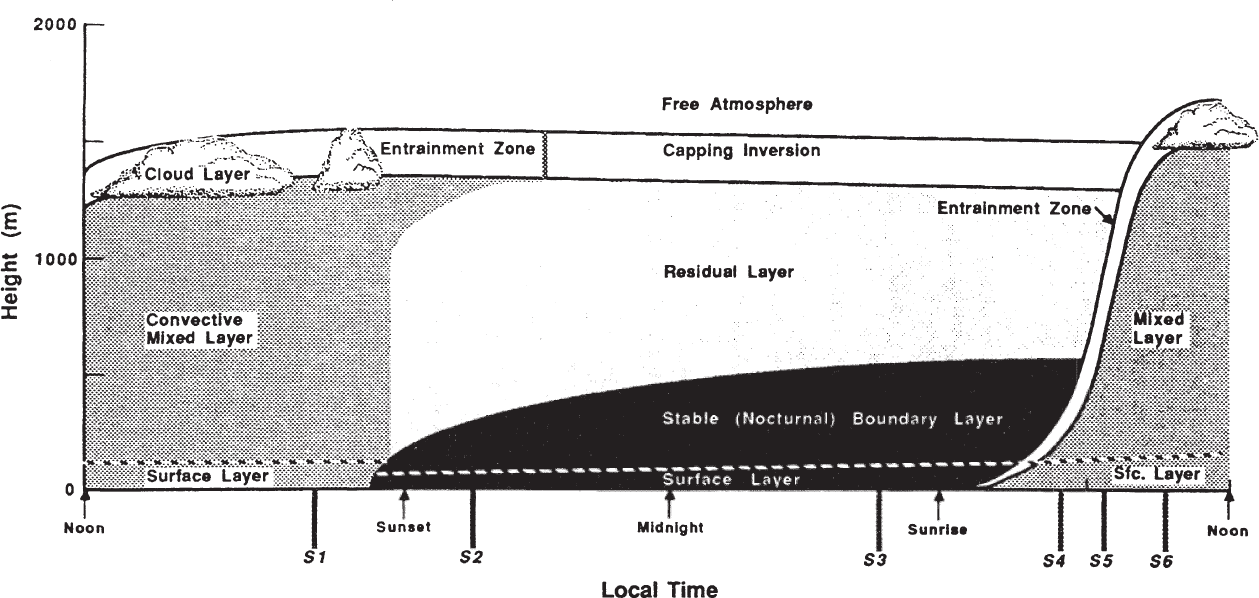
\includegraphics[width=0.9\textwidth]{fig/abl_stull.png}
    \caption{Diagram of the daily evolution of the structure of the ABL. Image based on \cite{stull2012introduction}.}
    \label{fig:ABL_structure}
  \vspace{-5pt}
\end{figure}

The figure~\ref{fig:ABL_structure} shows the structure and temporal evolution of the ABL, its components are the mixing layer, the residual layer and the stable boundary layer. Each of these has special characteristics and different physical processes that distinguish them. To understand the dynamics of the planetary boundary layer it is necessary to define each of them. However, in this study, we focus mostly on the stable nocturnal boundary layer, because is during the occurrence of this layer that katabatic winds form~\citep{poulos2008observational, stull2012introduction}.

\subsubsection{Stable boundary layer}
The stable nocturnal boundary layer is formed during the night when the sunlight stops reaching the ground. This layer is characterised by sporadic turbulence caused by wind shear and the contact with the surface, with a tendency to suppress turbulence. The upper limit of the stable boundary layer is located at the height where the intensity of the turbulence is a small fraction of its surface value. The air in this layer is statically stable, opposed as its daytime equivalent, the mixed layer~\citep{stull2012introduction}.

When the stable boundary layer is formed, the air that is close to the ground cools down and can form drainage winds or katabatic winds, only if there is a slope in the topography.

\subsection{Katabatic wind}

The katabatic winds are local winds that are created in presence of a descending terrain gradient when air masses flow downslope, continuously being cooled by radiative processes near the ground. They are a ventilation mechanism in mountainous regions~\citep{manins1979model}. Normally, these winds are shallow, where the thickness of the jet can go from 2 to 20~m. They have velocities on the order of 1 to 5~m/s \citep{stull2012introduction}. 

\begin{figure}[ht!]
	\vspace{-5pt}
    \centering
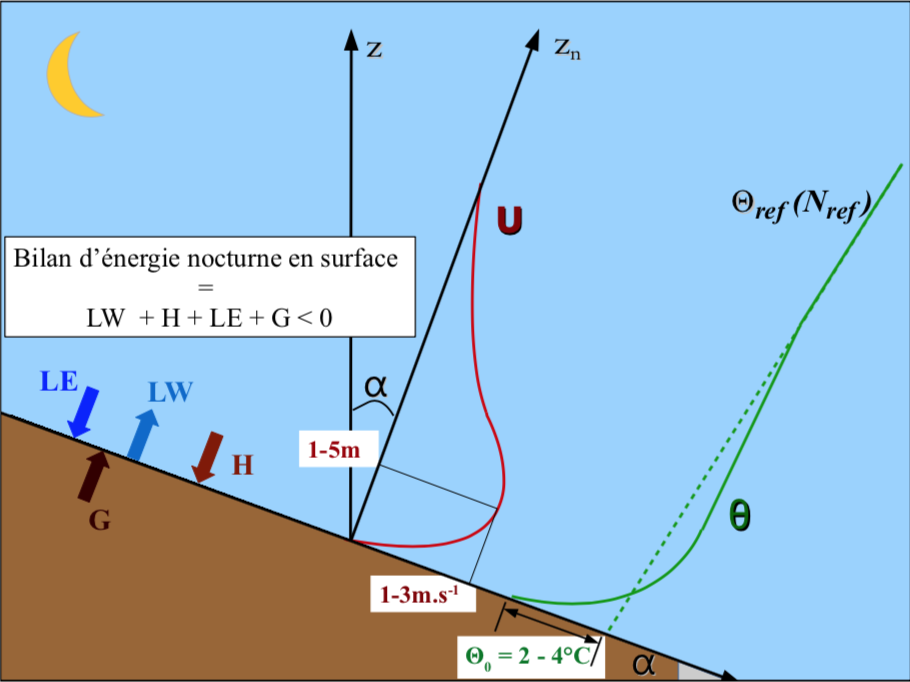
\includegraphics[width=0.6\textwidth]{fig/profiles_katabatic_wind.png}
    \caption{Characteristic wind profile (red) and potential profile (green) of the katabatic wind. Image from~\cite{claudine}.}
    \label{fig:u_profile}
  \vspace{-5pt}
\end{figure}

These winds are characterised for having a velocity profile as the one shown in the red curve in figure~\ref{fig:u_profile}. We can see that near the surface the velocity grows as we go up until it reaches a maximum and starts to decrease. This is the theoretical velocity profile of the katabatic winds. Also in figure~\ref{fig:u_profile}, we can see in the green curve the profile for the potential temperature, where we the theoretical profile shows that it grows rapidly as we go up until a point were it remains constant. This theoretical results can be useful to detect the occurrence of katabatic wind in the data sets.

An important factor to highlight about the katabatic winds is that external factors like synoptic or mesoscale winds can alter or destroy this kind of local winds~\citep{stull2012introduction}. The katabatic winds are important under conditions of slack synoptic pressure gradients~\citep{manins1979katabatic}. This factor plays an important role in the planning out the field campaign because we want to measure the katabatic jet as undisturbed as possible. For this, we are looking for a meteorological window when anticyclonic conditions will be present. 

\subsection{Turbulence Kinetic Energy (TKE)}
The TKE is defined as the kinetic energy per unit mass. This is one of the most important quantities to characterise turbulence in a flow, by giving us information about whether a region will become more turbulent, or whether turbulence will decay~\citep{stull2012introduction}.  Is defined as:

\begin{equation}
    e = \frac{1}{2} \big(\overline{u'^2} + \overline{v'^2} + \overline{w'^2}\big). 
    \label{eq:tke}
\end{equation}

\noindent where $e$ is the definition of turbulent kinetic energy (TKE). Is the sum of the variances of the wind components fluctuation. The over-line represents the average of the variable. 

\subsection{Covariance}

Recalling the classical definition of covariance between to variables, we have the relation 

\begin{equation}
    \text{covar}(A,B) = \frac{1}{N}\sum_{i=0}^{N-1} (A_i - \overline{A})(B_i - \overline{B}).
\end{equation}

\noindent Using the Reynolds averaging method in the previous expression we get:

\begin{subequations}
\begin{align}
    \text{covar}(A,B) &= \frac{1}{N}\sum_{i=0}^{N-1} a_i' b_i', \\
    &= \overline{a'b'}.
\end{align}
\end{subequations}

\noindent This is the mathematical definition of covariance. The covariance indicates the degree of common relationship between two variables. Is the principle by which we define the eddy fluxes.

\subsection{Eddy Flux}
According to \cite{stull2012introduction}, a turbulent flux or eddy flux is the transport of a physical quantity by the effect of the turbulence. In this project, we are mostly concerned with the sensible heat flux and the momentum flux. The sensible heat flux is given by the expression:

\begin{equation}
    H = \rho \ C_p \ \overline{w'\theta'},
\end{equation}

\noindent where $C_p$ is the specific heat at constant pressure and $\theta '$ is the fluctuations in potential temperature. We are interested in the vertical flux of the sensible heat, that is why we use the vertical wind fluctuation $w'$.

The momentum flux is given by the expression

\begin{equation}
    F = \rho \ \overline{u'w'}, 
\end{equation}

\noindent where $\rho$ is the density of air, and $u'$ and $w'$ are the fluctuations of velocity in the x-coordinate and in the vertical coordinate. The x-coordinate follows the slope and the z-coordinate is perpendicular to the slope. The latter expression also is known as a component of the \textbf{Reynolds stress tensor}. The Reynolds stress describes all the components of the momentum flux in a control volume.
